\chapter{Evolución y Comparación de la Blue Straggler}

Una vez la simulación de la interacción entre la estrella de $2 M_\odot$ y la de $1 M_\odot$ (nuestra blue straggler ahora), esta simulación se deja de lado: no tiene sentido alguno continuar evolucionando dos estrellas que no van a voler a interactuar, especialmente cuando no estamos interesados en la física de una de ellas.

Por lo tanto, se toma la última \texttt{PHOTO} creada por MESA (una \texttt{PHOTO} es un archivo de volcado binaro que guarda el estado completo de una estrella en un punto en concreto de la simulación), y se utiliza como punto de partida de una simulación secundaria, consiguiendo así la historia completa de la Blue Straggler antes de la TAMS.

\section{Evolución de Estrellas Similares}

Dado que, en una observación fotométrica, a menudo solo conocemos con certeza la luminosidad y temperatura de las estrellas observadas, naturalmente vamos a comparar nuestra Blue Straggler con estrellas simples que se encuentren en el mismo punto del diagrama HR, permitiéndonos de esta forma comprobar las diferencias entre la hipótesis aislada y la binaria. Para ver cómo se posiciona nuestra estrella en comparación con estrellas de masa similar durante su evolución, es necesario evolucionar una cuadrícula de estrellas en un intervalo de masas que englobe la masa de la Blue Straggler (ya que esperamos que evolucionen de manera similar).

Para ello, se emplea el repositorio \texttt{wsssss} \textit{(Walter's Set of Scripts for Studying Simulated Stars)} \citep{wsssss}, el cual contiene una serie de scripts muy útiles para crear y simular de forma simultánea cuadrículas de estrellas con MESA, actuando como una ``envoltura'' al código de simulación.

La evolución de esta cuadrícula de estrellas simulada y de la Blue Straggler puede verse en la figura \ref{fig:sim_estrellas}

Se aprecia cómo la Blue Straggler evoluciona a temperaturas superiores que estrellas similares en masa (como es el caso de la estrella de $1.82 M_\odot$), fruto de su estructura interior rejuvenecida.

\begin{figure}[H]
  \centering
  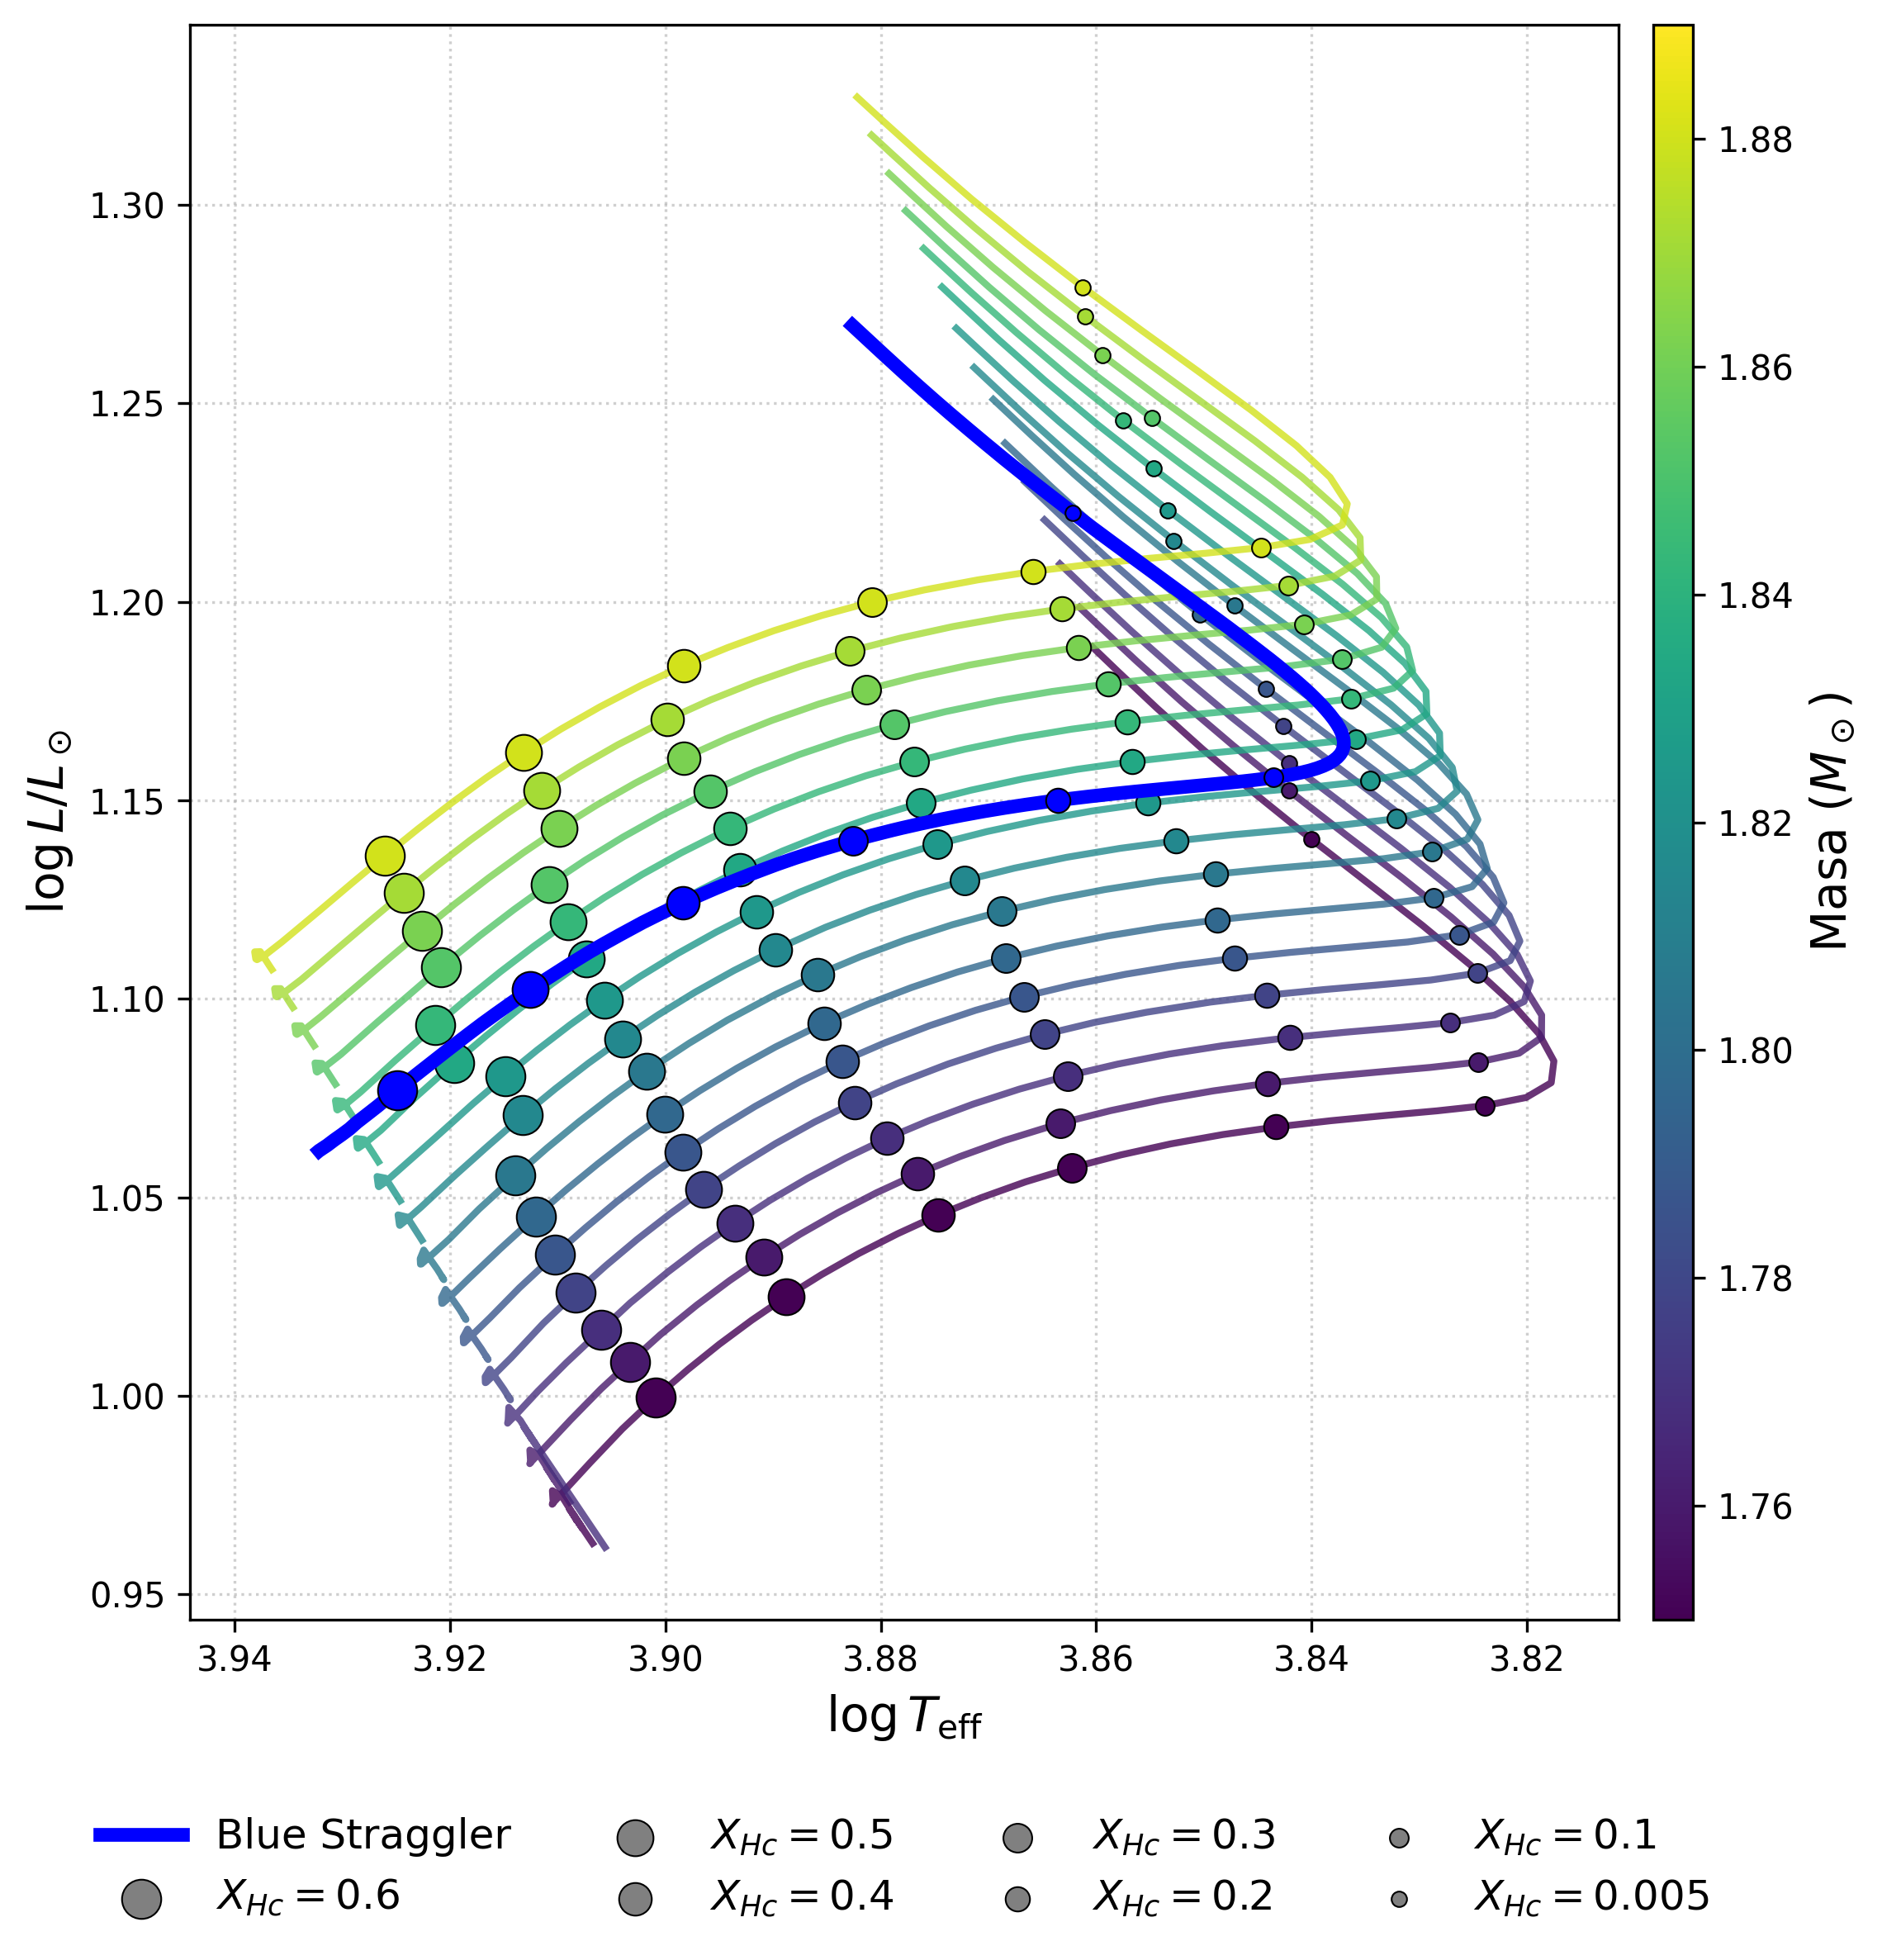
\includegraphics[width=\linewidth]{Imagenes/mass_grid_comparison.png}
  \caption{Trazas en el diagrama HR de distintas estrellas con masas desde $1.75 M_\odot$ hasta $1.90 M_\odot$. Se incluye la traza de la Blue Straggler en azul. En cada traza se han representado diversos puntos, correspondientes a los valores indicados de la fracción de hidrógeno en el núcleo de cada estrella.}
  \label{fig:sim_estrellas}
\end{figure}

Resulta interesante comparar el interior de la Blue Straggler con el de una estrella de masa similar. Podemos ver esto con un diagrama de Kippenhahn (Figura \ref{fig:kippenhahn_comparison}).

\begin{figure}[H]
  \centering
  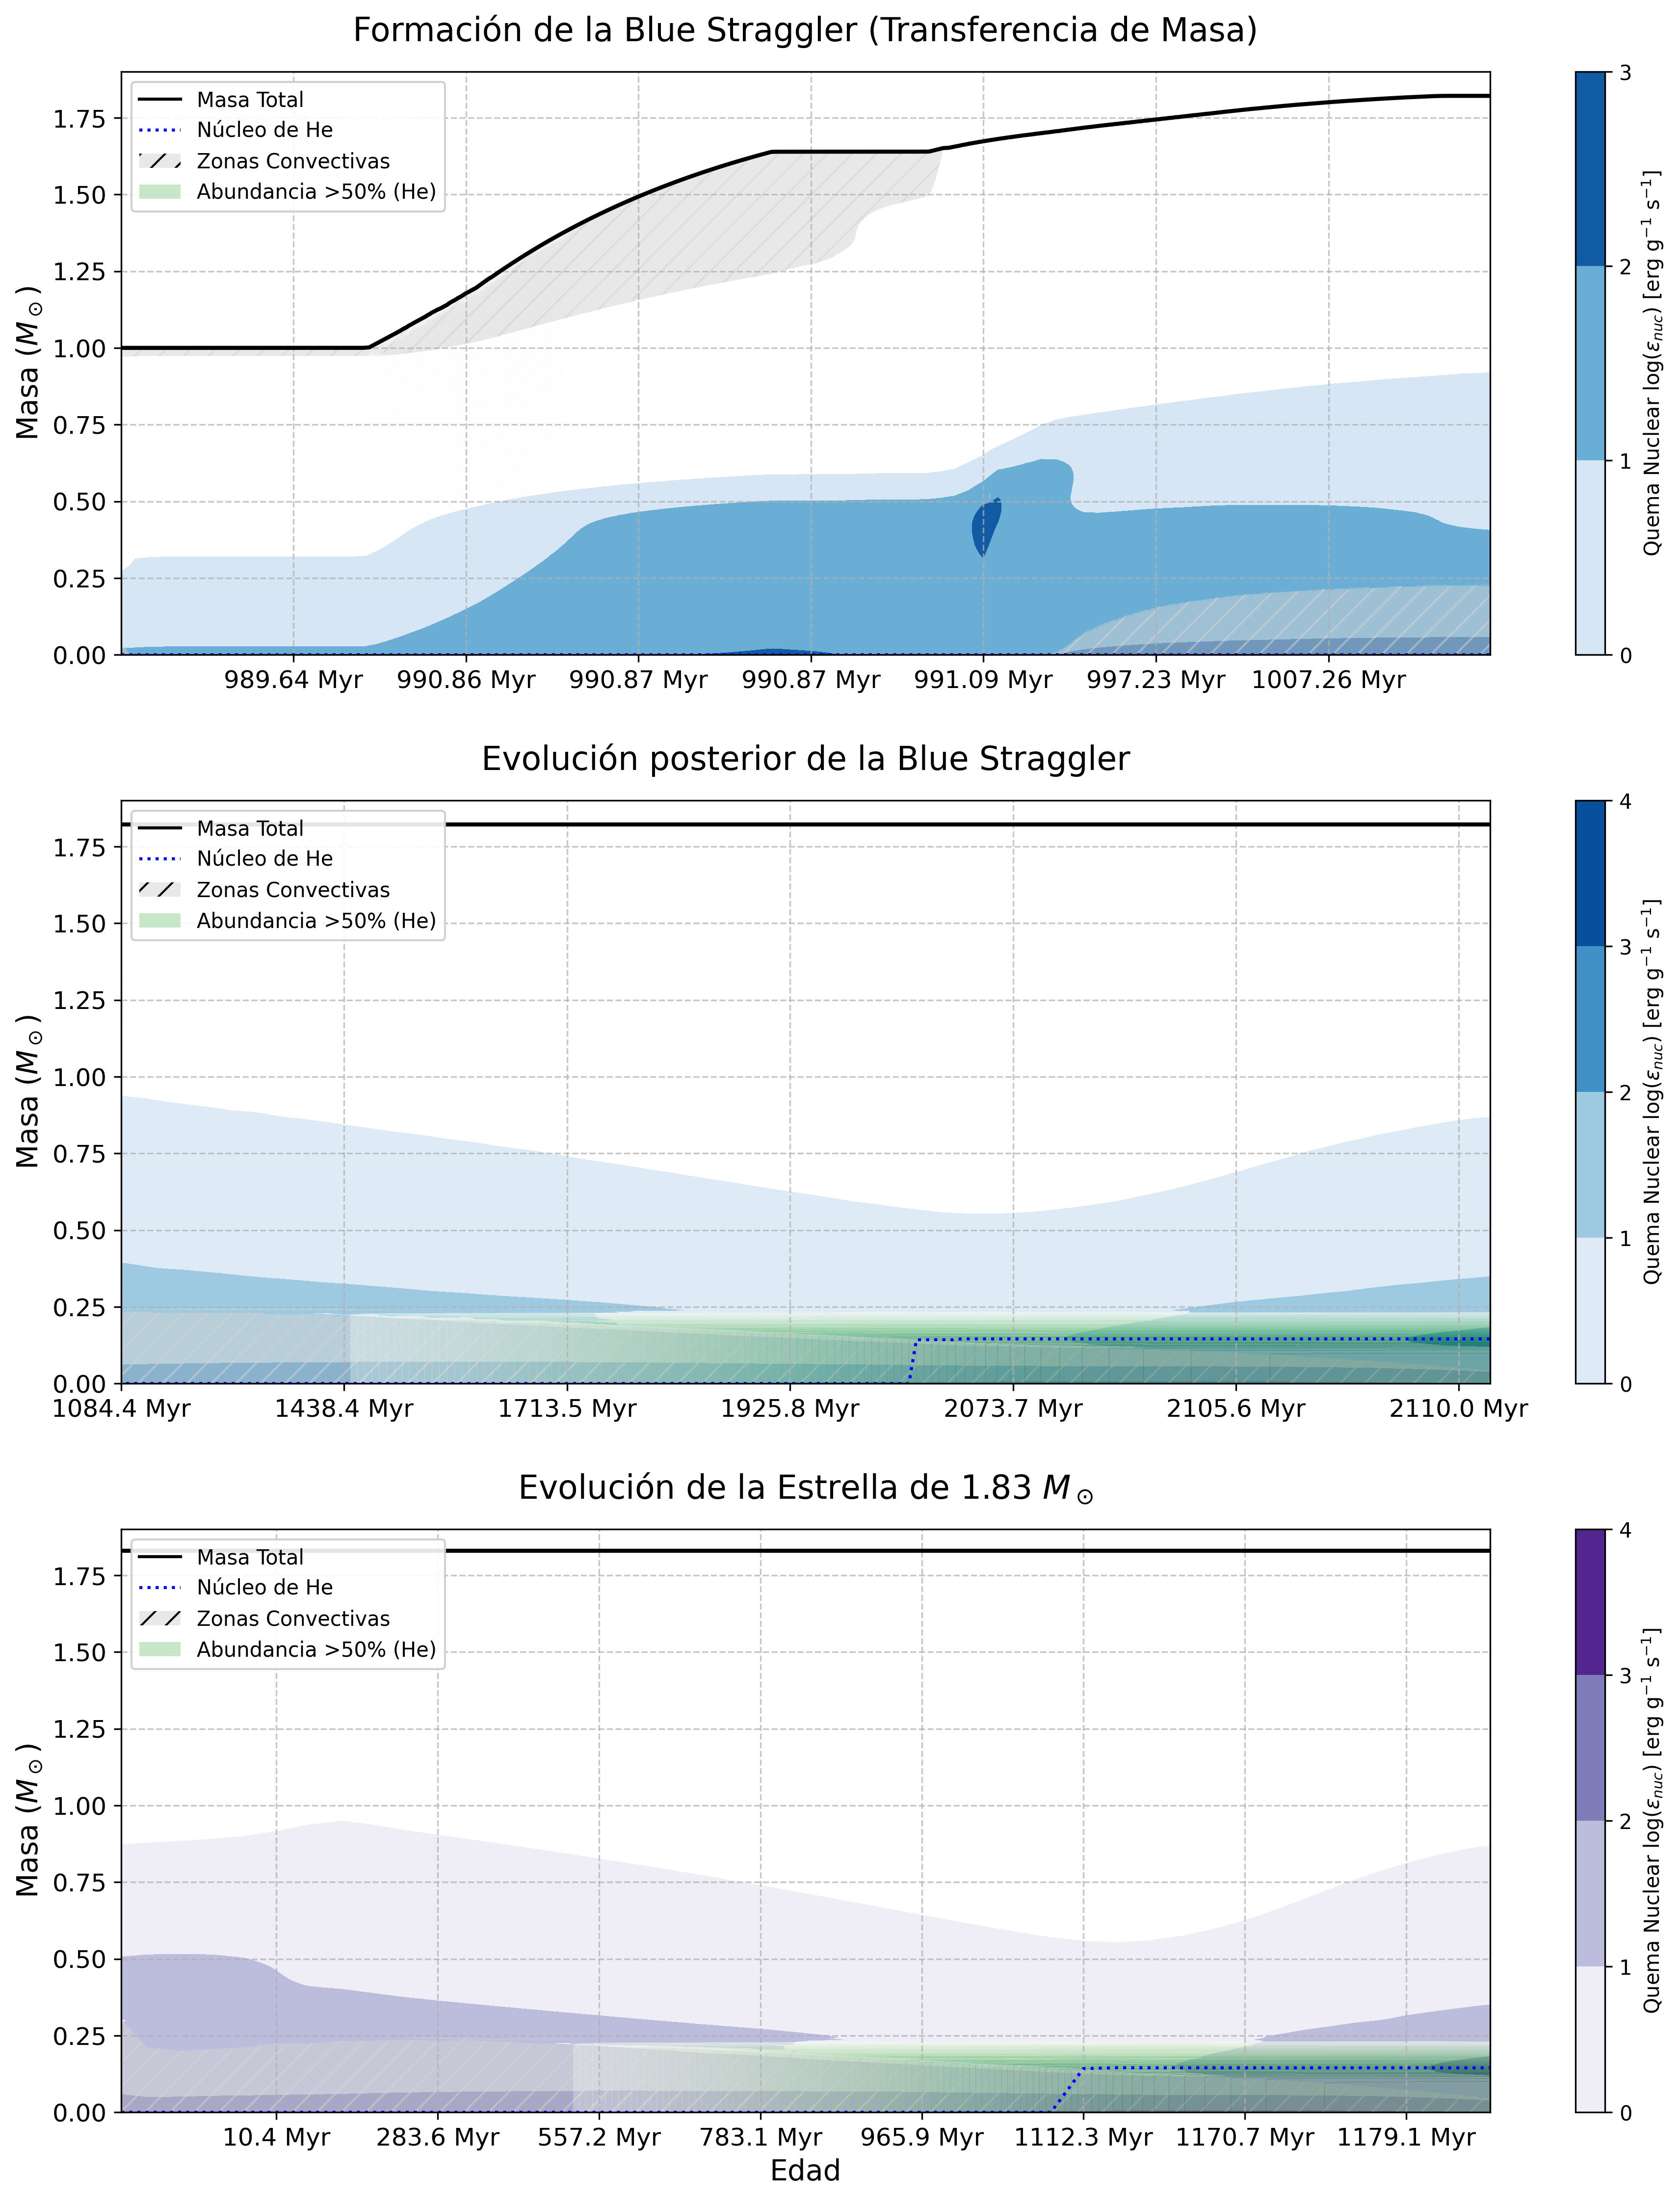
\includegraphics[width=0.95\linewidth]{Imagenes/kippenhahn_comparision.png}
  \caption{Diagrama de Kippenhahn de la Blue Straggler (arriba) y de una estrella de $1.83 M_\odot$ (abajo). El diagrama de la Blue Straggler ha sido dividido en pre y post-transferencia de masa. Se muestra la intensidad del quemado nuclear mediante el color, las zonas de convección mediante el sombreado gris y la abundancia de helio con el sombreado verde. Por último, se ha representado la masa total y el núcleo de helio con la línea azul punteada.}
  \label{fig:kippenhahn_comparison}
\end{figure}

Puesto que la Blue Straggler ya había evolucionado ligeramente al inicio de su vida, se pueden apreciar ligeras diferencias en su estructura interior, en comparación con la estrella de $1.83 M_\odot$.

\section{Comparación Astrosismológica}

El objetivo final de este trabajo es determinar si la astrosismología puede ayudarnos a identificar los escenarios de evolución binaria que dan lugar a las Blue Stragglers, frente a la evolución estelar simple. Para ello, en esta sección se lleva a cabo un estudio comparativo entre las frecuencias de oscilación de la Blue Straggler y de las estrellas de la cuadrícula de la sección anterior.
\subsection{Gran Separación}

Una primera aproximación consiste en calcular la gran separación $\Delta\nu$ para las frecuencias de oscilación de la Blue Straggler y de las estrellas de la cuadrícula. Esta se define como la diferencia de frecuencia entre modos de idéntico orden y harmonicidad (es decir, $\nu_{n_{pg}}^l - \nu_{n_{pg}-1}^l$). Un ejemplo de esta gran separación puede verse en la Figura \ref{fig:great_separation}.

\begin{figure}[H]
  \centering
  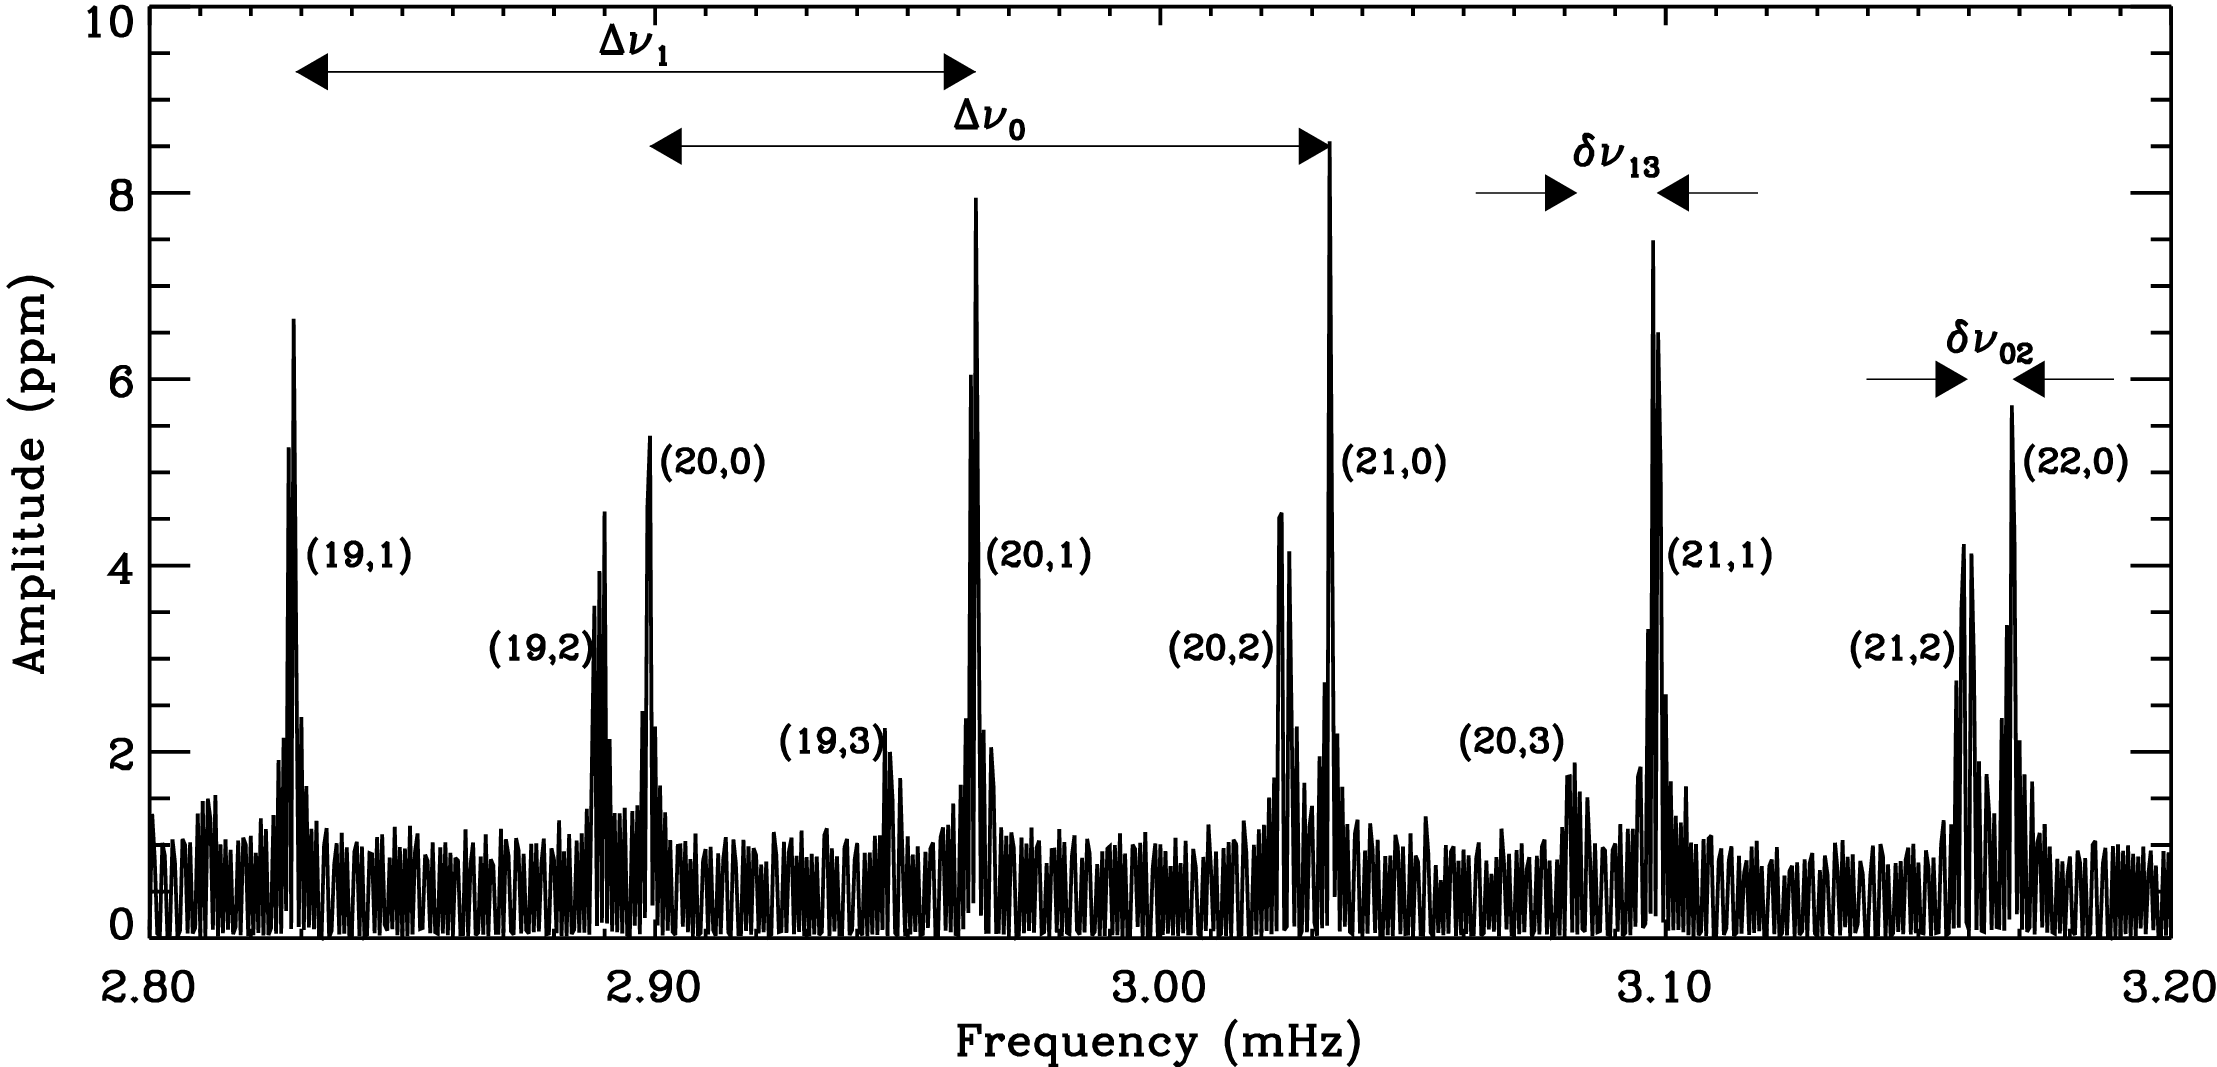
\includegraphics[width=0.95\linewidth]{Imagenes/virgo-detail.png}
  \caption{Detalle del espectro de oscilaciones solares, observado por VIRGO. Cada pico de frecuencia está anotado con su valor de $n$ y $l$ correspondiente. Se indican también las grandes y pequeñas separaciones de frecuencia, representadas como $\Delta\nu$ y $\delta\nu$, respectivamente. (La pequeña separación de frecuencias, $\delta\nu$, se define como $\nu_{n_{pg}}^l - \nu_{n_{pg}}^{l+2}$). Imagen tomada de \citet{Bedding_2003}.}
  \label{fig:great_separation}
\end{figure}

Para nuestro caso en particular, emplearemos la siguiente notación: $\Delta \nu_k = \nu_{-10 + k + 1}^l - \nu_{-10 + k}^l$, de modo que $\Delta \nu_0 = \nu_{-9}^l - \nu_{-10}^l$, $\Delta \nu_1 = \nu_{-8}^l - \nu_{-9}^l$, y así sucesivamente.

Podemos, pues, representar la gran separación $\Delta \nu$ de las estrellas de nuestra cuadrícula y la de la Blue Straggler en el mismo gráfico, para observar sus diferencias.

\clearpage
\newgeometry{left=1.5cm, right=1.5cm, top=1.5cm, bottom=2.5cm}
\thispagestyle{plain}

\begin{figure}[H]
  \centering
  
\includegraphics[width=\linewidth]{Imagenes/great_separations_hand_picked/great_separation_mass_1.84_pcomp_4_pbs_5_H_69.7.png}
  \label{fig:great_separation_69.7}

  \vspace{-1.05cm}
  
\includegraphics[width=\linewidth]{Imagenes/great_separations_hand_picked/great_separation_mass_1.84_pcomp_16_pbs_29_H_46.0.png}
  \label{fig:great_separation_46.0}

  \vspace{-1.05cm}
  
\includegraphics[width=\linewidth]{Imagenes/great_separations_hand_picked/great_separation_mass_1.836_pcomp_20_pbs_40_H_35.7.png}
  \label{fig:great_separation_35.7}

  \vspace{-1.05cm}
  
\includegraphics[width=\linewidth]{Imagenes/great_separations_hand_picked/great_separation_mass_1.834_pcomp_24_pbs_51_H_25.6.png}
  \label{fig:great_separation_25.6}

  \vspace{-1.05cm}
  
\includegraphics[width=\linewidth]{Imagenes/great_separations_hand_picked/great_separation_mass_1.832_pcomp_28_pbs_63_H_14.8.png}
  \label{fig:great_separation_14.8}
\end{figure}

\clearpage
\thispagestyle{plain}
\begin{figure}[H]
  \centering
  
\includegraphics[width=\linewidth]{Imagenes/great_separations_hand_picked/great_separation_mass_1.79_pcomp_38_pbs_72_H_0.8.png}
  \label{fig:great_separation_0.8}

  \vspace{-1.05cm}
  
\includegraphics[width=\linewidth]{Imagenes/great_separations_hand_picked/great_separation_mass_1.79_pcomp_45_pbs_92_H_0.1.png}
  \label{fig:great_separation_0.1}
  \vspace{-0.5cm}

  
\includegraphics[width=0.9\linewidth]{Imagenes/great_separations_hand_picked/global_hr_diagram.png}
  \label{fig:global_hr_diagram}
  \vspace{-0.4cm}
  \caption{Comparación de la gran separación $\Delta\nu$ en función del índice $k$ para los modos $l=0, 1, 2$ (paneles de la página anterior y superiores). Se compara el modelo de la Blue Straggler (triángulos) con estrellas de evolución estándar (círculos) en distintos puntos de la secuencia principal, ordenados en el tiempo. Panel inferior: Diagrama HR mostrando la traza evolutiva de la Blue Straggler (azul) junto a las trazas de las estrellas estándar comparadas. Los pares de perfiles concretos empleados en cada comparación están resaltados con sus respectivos marcadores, numerados del 1 al 7.}
\end{figure}

\clearpage
\restoregeometry

Resulta interesante observar cómo las diferencias más marcadas en $\Delta\nu$ entre la Blue Straggler y las estrellas de evolución estándar se dan en los modos de orden $l=2$ para todas las etapas de evolución, mientras que estas son apenas observables para modos con orden $l=0$. Además, las diferencias para $l=2$ y $l=1$ se vuelven mayores en etapas evolutivas posteriores de la Blue Straggler, mientras que estas decrecen para $l=0$.

Las diferencias máximas observadas en la gran separación para cada modo, restringidas a los órdenes radiales $n_{pg} \in [-10, 10]$ ($\Delta \nu_0$ a $\Delta \nu_{20}$), se cuantifican en la Tabla \ref{tab:max_diff_dnu}.

\begin{table}[htpb]
  \centering
  \begin{tabular}{
      c
      S[table-format=2.1, table-space-text-post=\%]
      c
      c
      c
      S[table-format=2.1]
    }
    \toprule
    & & \multicolumn{3}{c}{$|\Delta(\Delta\nu)|_\mathrm{max}$ (ciclos\,día$^{-1}$)} & \\
    \cmidrule(lr){3-5}
    {Par} & {$H_c$ (\%)} & {$l = 0$} & {$l = 1$} & {$l = 2$} & {$r = l{=}2/l{=}0$} \\
    \midrule
    Par 1 ($1.840\,M_\odot$) & 69.7 & 0.0826 & 0.469 & 0.863 & 10.4 \\
    Par 2 ($1.840\,M_\odot$) & 46.0 & 0.0563 & 0.827 & 1.412 & 25.1 \\
    Par 3 ($1.836\,M_\odot$) & 35.7 & 0.0474 & 0.708 & 1.425 & 30.0 \\
    Par 4 ($1.834\,M_\odot$) & 25.6 & 0.0424 & 0.481 & 1.464 & 34.5 \\
    Par 5 ($1.832\,M_\odot$) & 14.8 & 0.0392 & 0.432 & 1.240 & 31.6 \\
    Par 6 ($1.790\,M_\odot$) &  0.8 & 0.0454 & 1.977 & 2.076 & 45.7 \\
    Par 7 ($1.790\,M_\odot$) &  0.1 & 0.0281 & 2.544 & 2.491 & 88.5 \\
    \bottomrule
  \end{tabular}
  \caption{Diferencia máxima absoluta en la gran separación $|\Delta(\Delta\nu)|_\mathrm{max}$ entre la Blue Straggler y la estrella de evolución estándar, para cada par de comparación y modo $l$. Cada par está emparejado a idéntica fracción de hidrógeno central $H_c$, de modo que las diferencias son de carácter puramente estructural. La última columna recoge la razón $r = |\Delta(\Delta\nu)|_\mathrm{max}^{l=2}\,/\,|\Delta(\Delta\nu)|_\mathrm{max}^{l=0}$, que cuantifica la mayor sensibilidad diagnóstica de los modos $l=2$ frente a los modos radiales.}
  \label{tab:max_diff_dnu}
\end{table}

Este intervalo de orden radial (entre $g_{10}$ y $p_{10}$) es un intervalo amplio que engloba pulsaciones de los modos $g$ y $p$ de bajo orden. Elegimos este intervalo pues se trata de la zona de oscilación esperada para las $\delta$ Scuti, zona donde se encuentra la Blue Straggler objetivo de nuestro estudio.

%Para garantizar que las diferencias observadas entre la Blue Straggler y las estrellas de evolución estándar reflejan diferencias estructurales genuinas (y no artefactos numéricos del código), es interesante realizar una prueba de control. Para ello, analizaremos las oscilaciones de dos estrellas regulares de masas muy similares ($1.832$ y $1.834\,$M$_\odot$) que evolucionan de forma casi idéntica en el diagrama HR. Si las desviaciones observadas anteriormente fuesen el resultado de inestabilidades del código, cabría esperar que también aparecieran diferencias notables al comparar estos dos modelos estándar.

%El resultado de esta prueba de control puede apreciarse en la Figura \ref{fig:control_great_separation}. Como se puede observar, las diferencias entre ambos modelos son muy pequeñas, lo que confirma que las diferencias observadas entre la Blue Straggler y las estrellas de evolución estándar son reales.

%\begin{figure}[p]
%  \centering
%  
\includegraphics[width=\linewidth]{Imagenes/great_separations_comp_1.832_1.834_hand_picked/great_separation_1.832_vs_1.834_p1_9_p2_9_H_64.5.png}

%  \vspace{-0.5cm}
%  
\includegraphics[width=\linewidth]{Imagenes/great_separations_comp_1.832_1.834_hand_picked/great_separation_1.832_vs_1.834_p1_27_p2_27_H_17.9.png}

%  \vspace{-0.5cm}
%  
\includegraphics[width=\linewidth]{Imagenes/great_separations_comp_1.832_1.834_hand_picked/great_separation_1.832_vs_1.834_p1_43_p2_43_H_0.1.png}

%  \vspace{0.5cm}
%  \begin{tabular}{
%      c
%      S[table-format=2.1, table-space-text-post=\%]
%      c
%      c
%      c
%      S[table-format=2.1]
%    }
%    \toprule
%    & & \multicolumn{3}{c}{$|\Delta(\Delta\nu)|_\mathrm{max}$ (ciclos\,día$^{-1}$)} & \\
%    \cmidrule(lr){3-5}
%    {Par} & {$H_c$ (\%)} & {$l = 0$} & {$l = 1$} & {$l = 2$} & {$r = l{=}2/l{=}0$} \\
%    \midrule
%    Par 1 & 64.5 & 0.0049 & 0.0586 & 0.1317 & 27.1 \\
%    Par 2 & 17.9 & 0.0210 & 0.1271 & 0.3998 & 19.1 \\
%    Par 3 &  0.1 & 0.0144 & 0.1244 & 0.1640 & 11.4 \\
%    \bottomrule
%  \end{tabular}

%  \vspace{0.2cm}
%  \caption{Prueba de control entre dos estrellas de evolución estándar con masas $1.832\,M_\odot$ (triángulos) y $1.834\,M_\odot$ (círculos). Los paneles muestran la comparación de la gran separación $\Delta\nu$ en función del índice $k$ para los modos $l=0, 1, 2$ en tres etapas distintas de la secuencia principal (de arriba a abajo: $H_c \approx 64.5\%$, $17.9\%$ y $0.1\%$). El patrón oscilatorio de ambas estrellas es prácticamente idéntico. En la tabla inferior se cuantifica la diferencia máxima absoluta en la gran separación, $|\Delta(\Delta\nu)|_\mathrm{max}$, obtenida entre ambos modelos para estos mismos puntos. Como se puede observar, las variaciones registradas son comparativamente inferiores a las encontradas al analizar la Blue Straggler (ver Tabla~\ref{tab:max_diff_dnu}), descartando cualquier inestabilidad numérica como su origen.}

%  \label{fig:control_great_separation}
%\end{figure}

\subsection{Frecuencias Individuales}

Otro indicador de las diferencias estructurales entre la Blue Straggler y las estrellas de evolución estándar es la comparación de las frecuencias individuales de los modos ($\nu^{\text{Ref}}_{n_{pg}, l} - \nu^{\text{BS}}_{n_{pg}, l}$). De igual manera que se hizo anteriormente con la gran separación, se puede representar esta diferencia para distintos puntos de la secuencia principal. En la figura \ref{fig:individual_frequencies_hand_picked} se muestran estos resultados para los mismos pares de perfiles que se han utilizado en las secciones anteriores.

\clearpage
\newgeometry{left=1.5cm, right=1.5cm, top=1.5cm, bottom=2.5cm}
\thispagestyle{plain}

\begin{figure}[H]
  \centering
  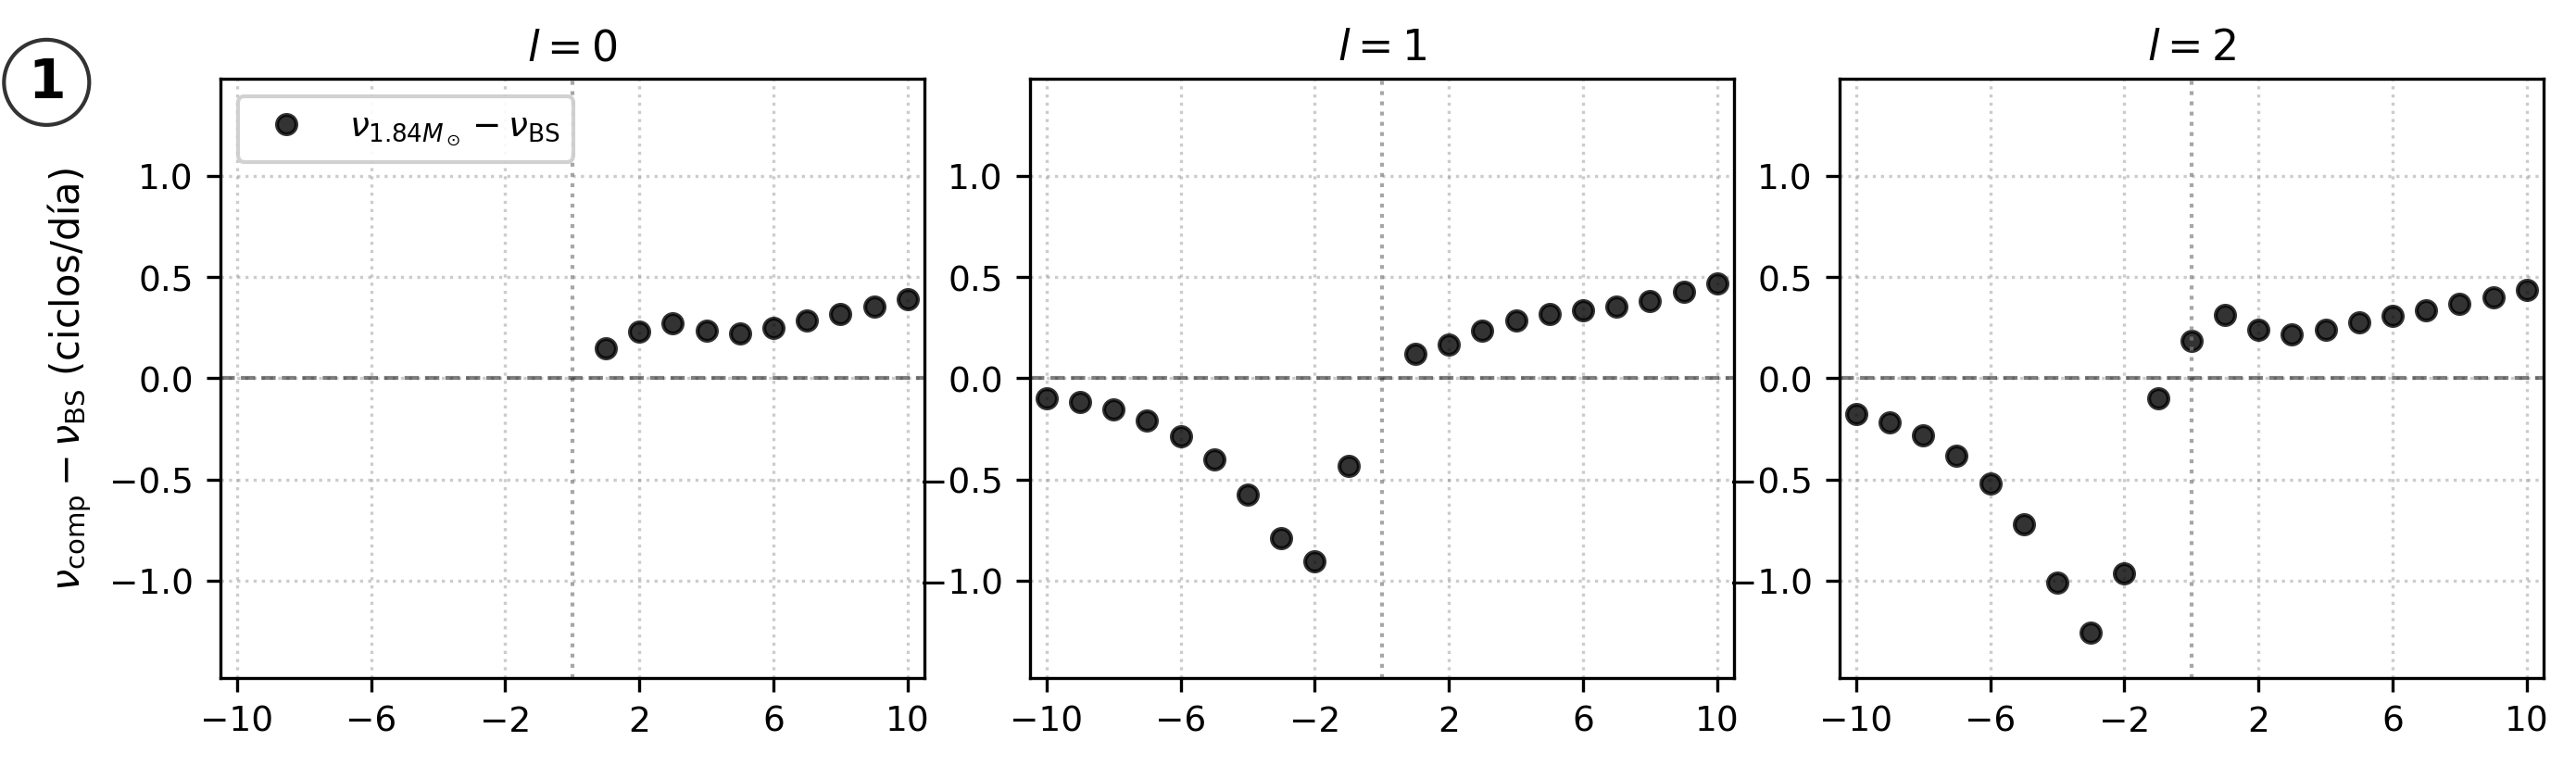
\includegraphics[width=\linewidth]{Imagenes/gyre_analysis_hand_picked/gyre_analysis_mass_1.84_pcomp_4_pbs_5_H_69.7.png}
  \label{fig:gyre_analysis_69.7}

  \vspace{-1.05cm}
  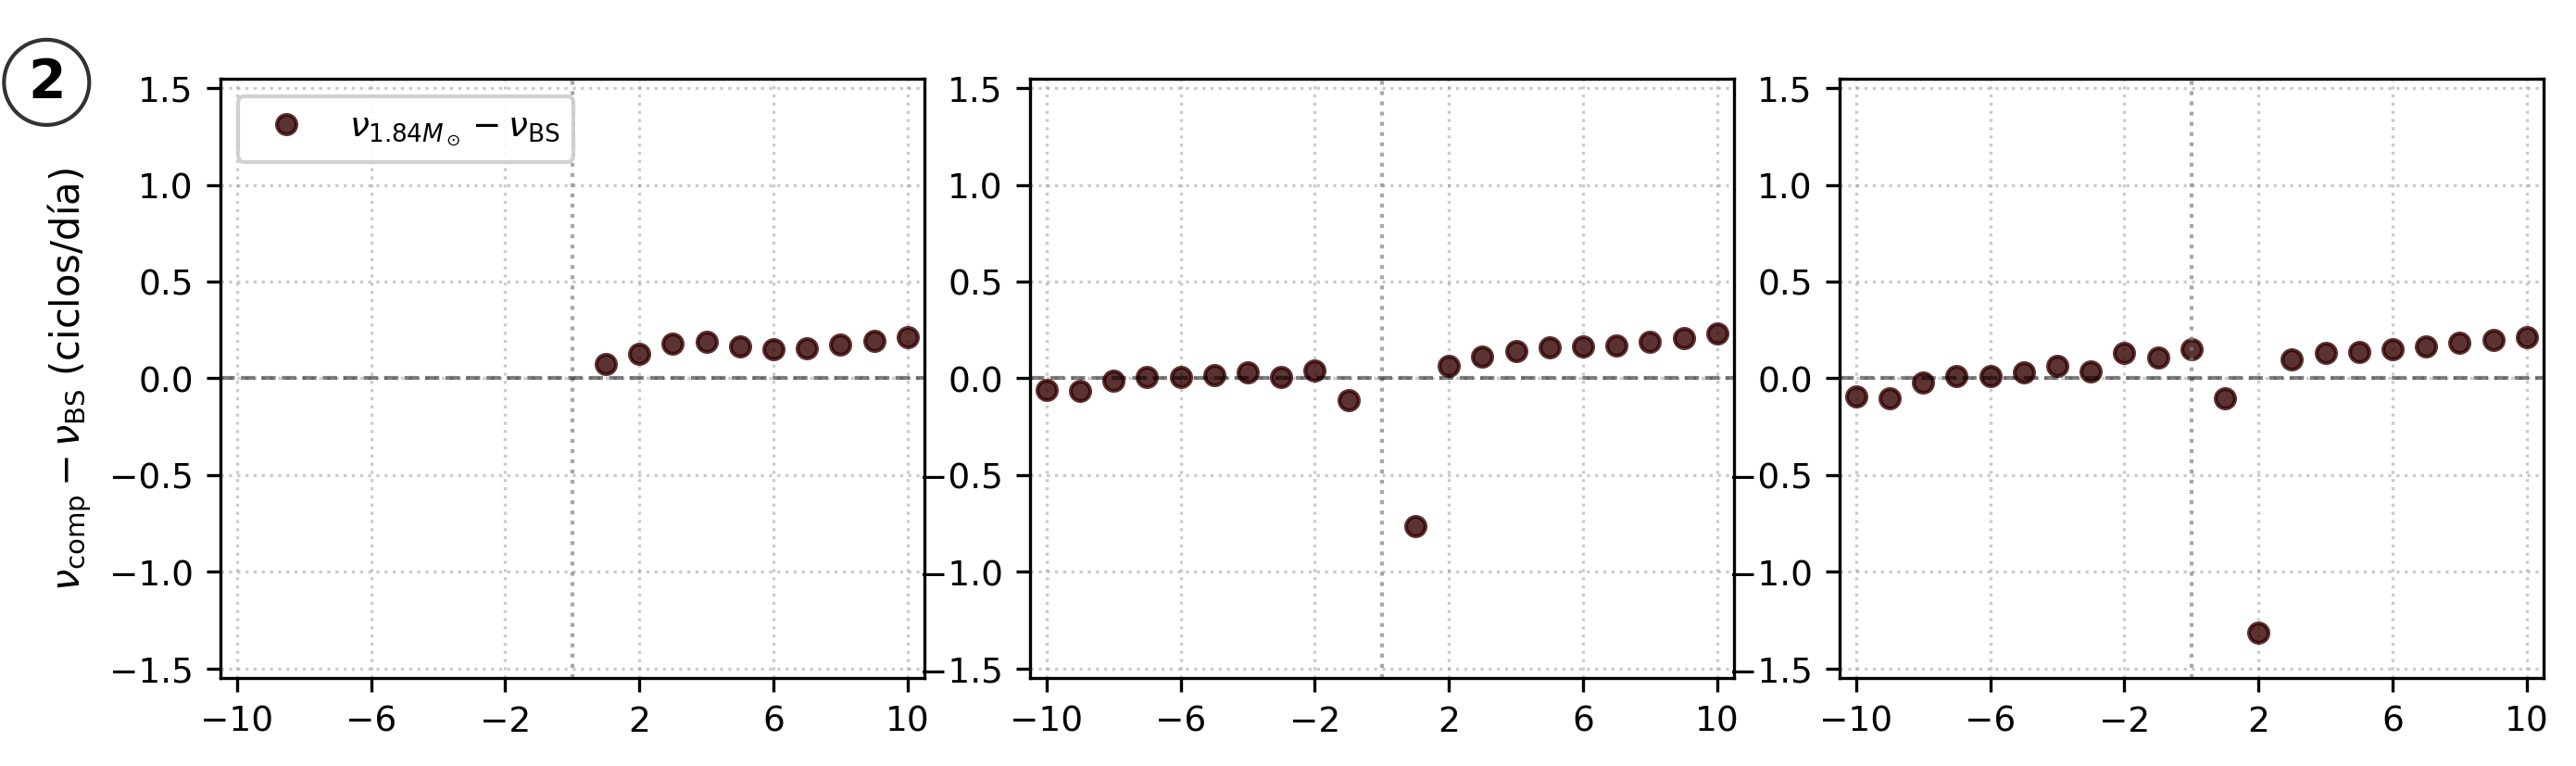
\includegraphics[width=\linewidth]{Imagenes/gyre_analysis_hand_picked/gyre_analysis_mass_1.84_pcomp_16_pbs_29_H_46.0.png}
  \label{fig:gyre_analysis_46.0}

  \vspace{-1.05cm}
  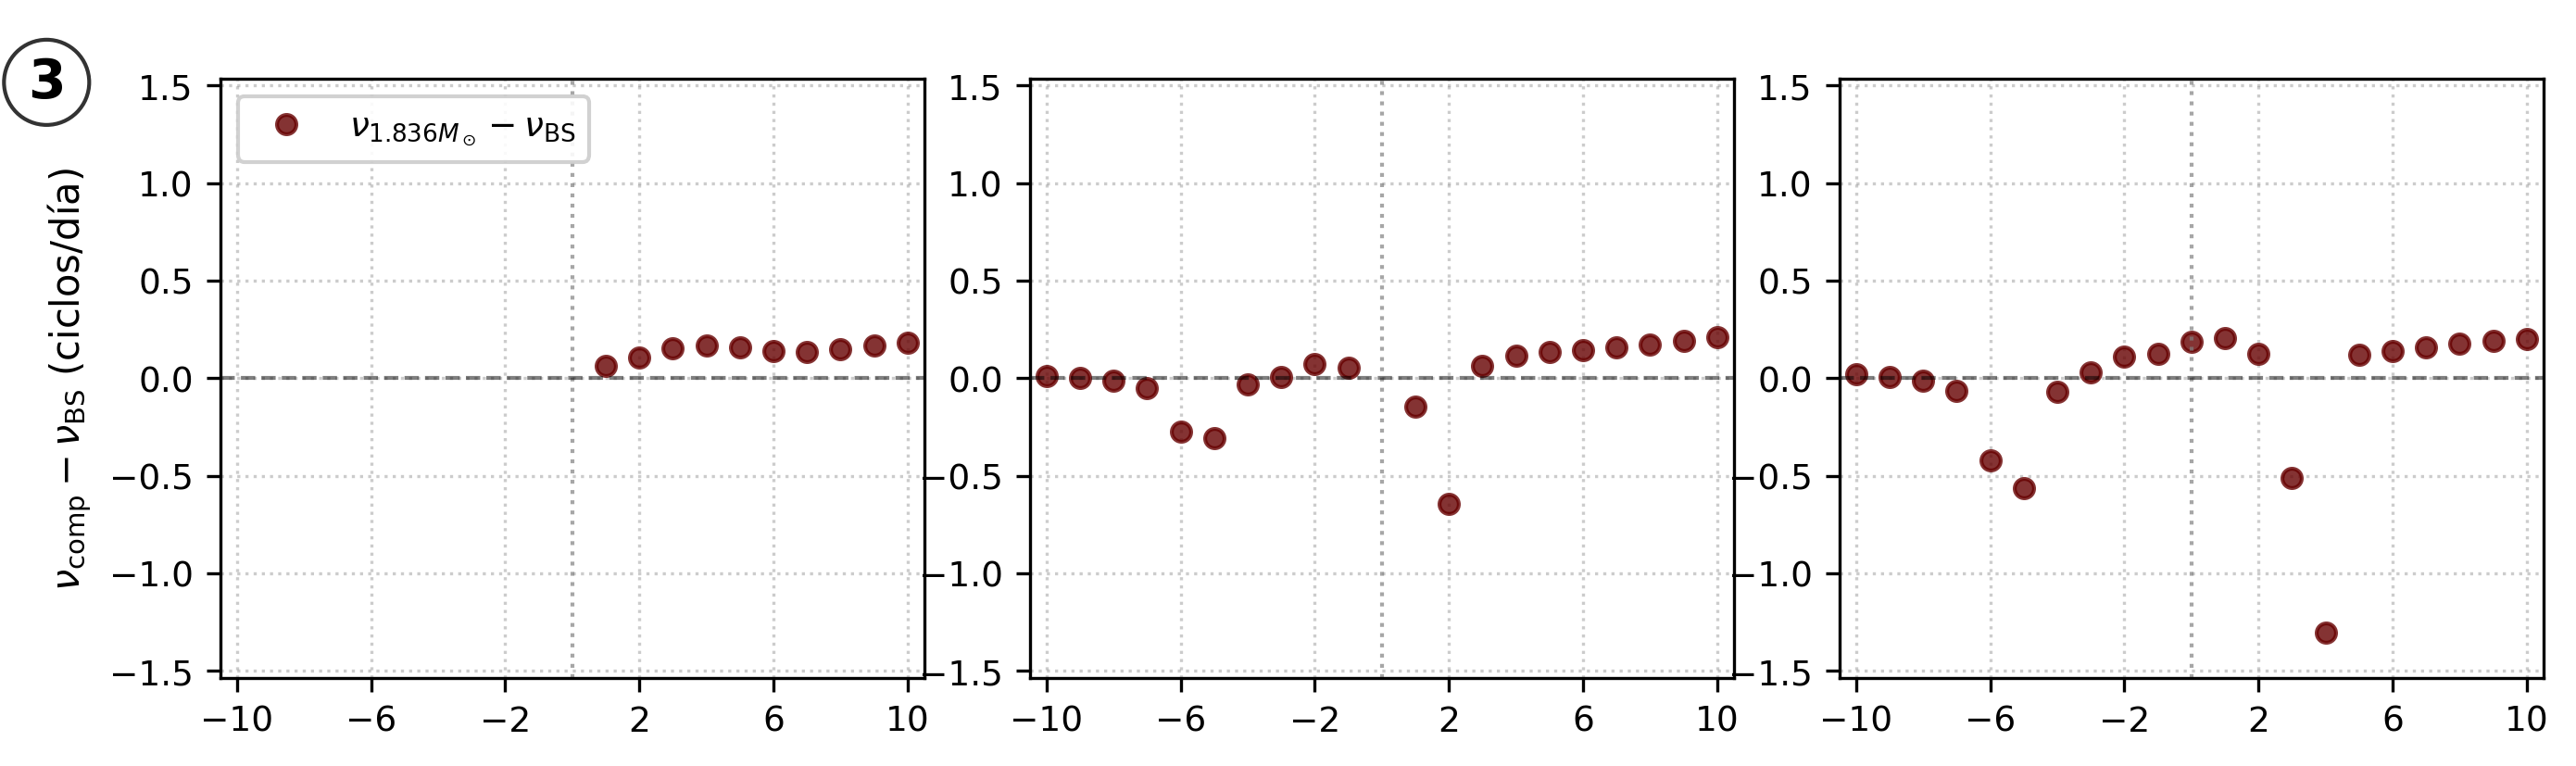
\includegraphics[width=\linewidth]{Imagenes/gyre_analysis_hand_picked/gyre_analysis_mass_1.836_pcomp_20_pbs_40_H_35.7.png}
  \label{fig:gyre_analysis_35.7}

  \vspace{-1.05cm}
  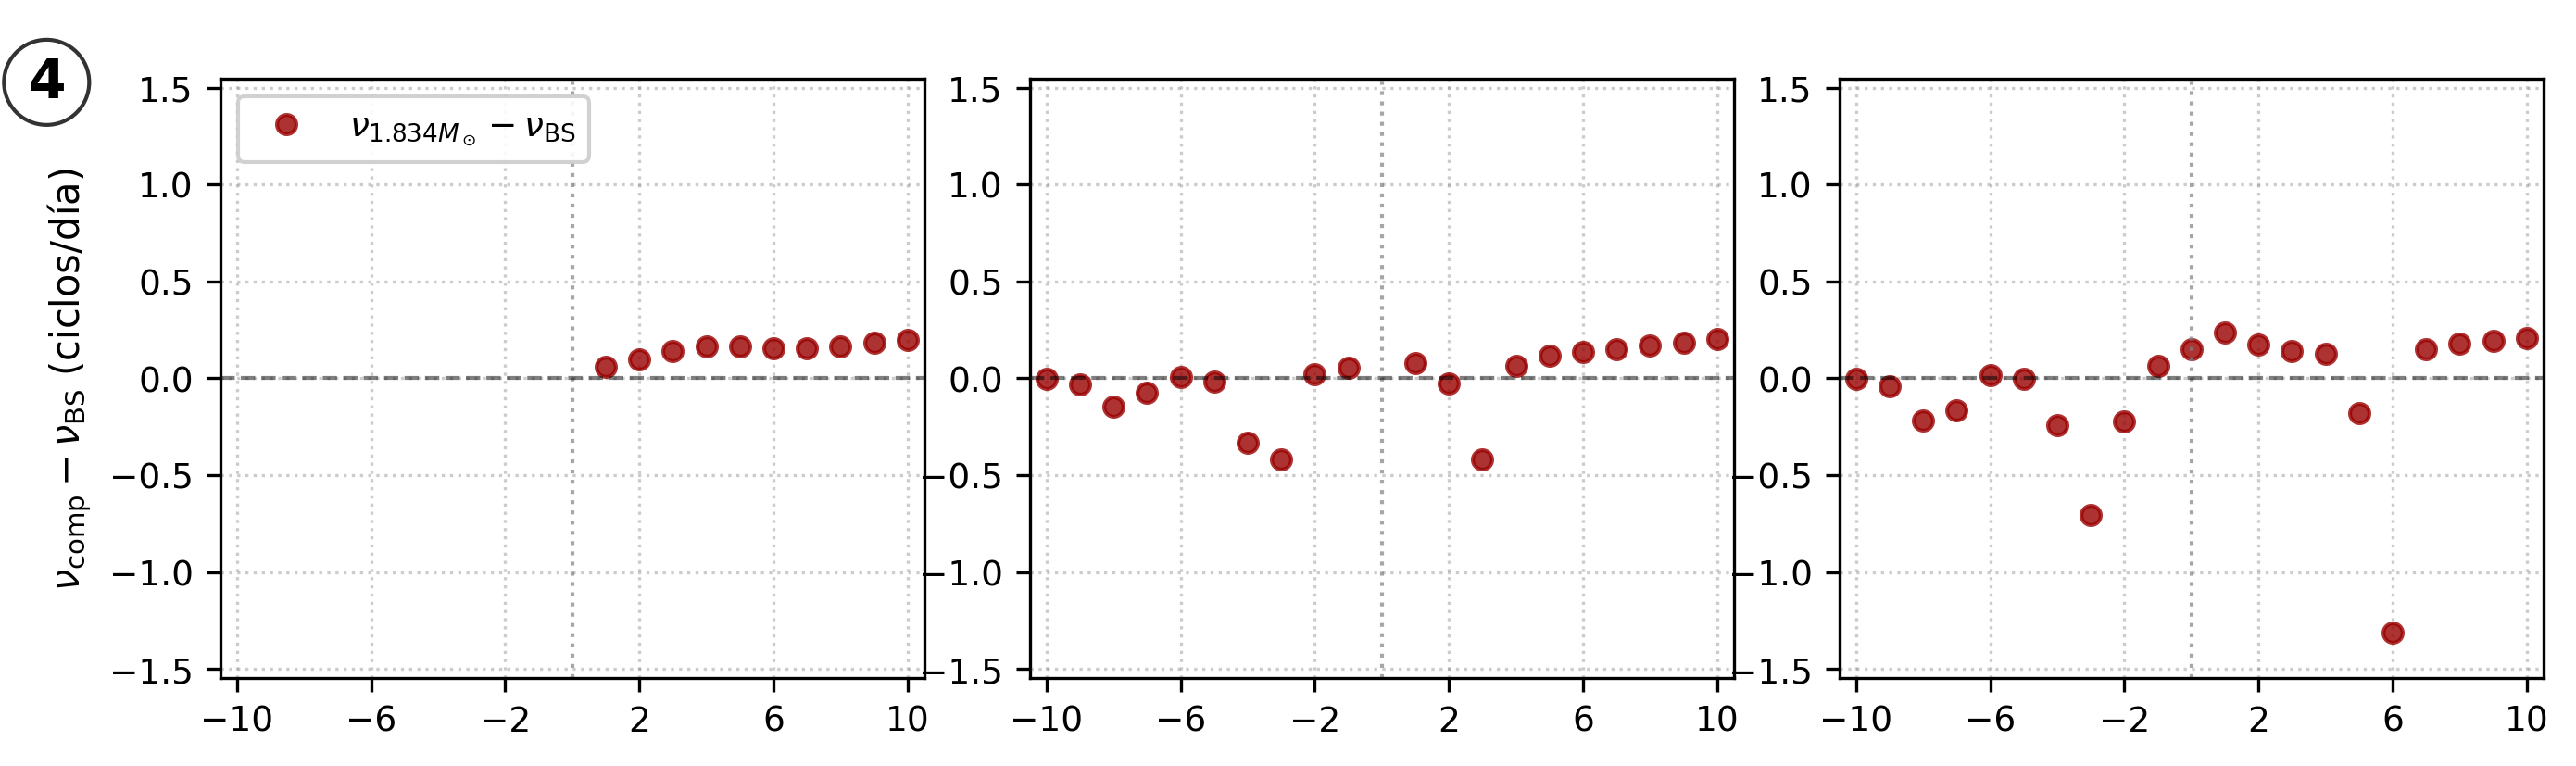
\includegraphics[width=\linewidth]{Imagenes/gyre_analysis_hand_picked/gyre_analysis_mass_1.834_pcomp_24_pbs_51_H_25.6.png}
  \label{fig:gyre_analysis_25.6}

  \vspace{-1.05cm}
  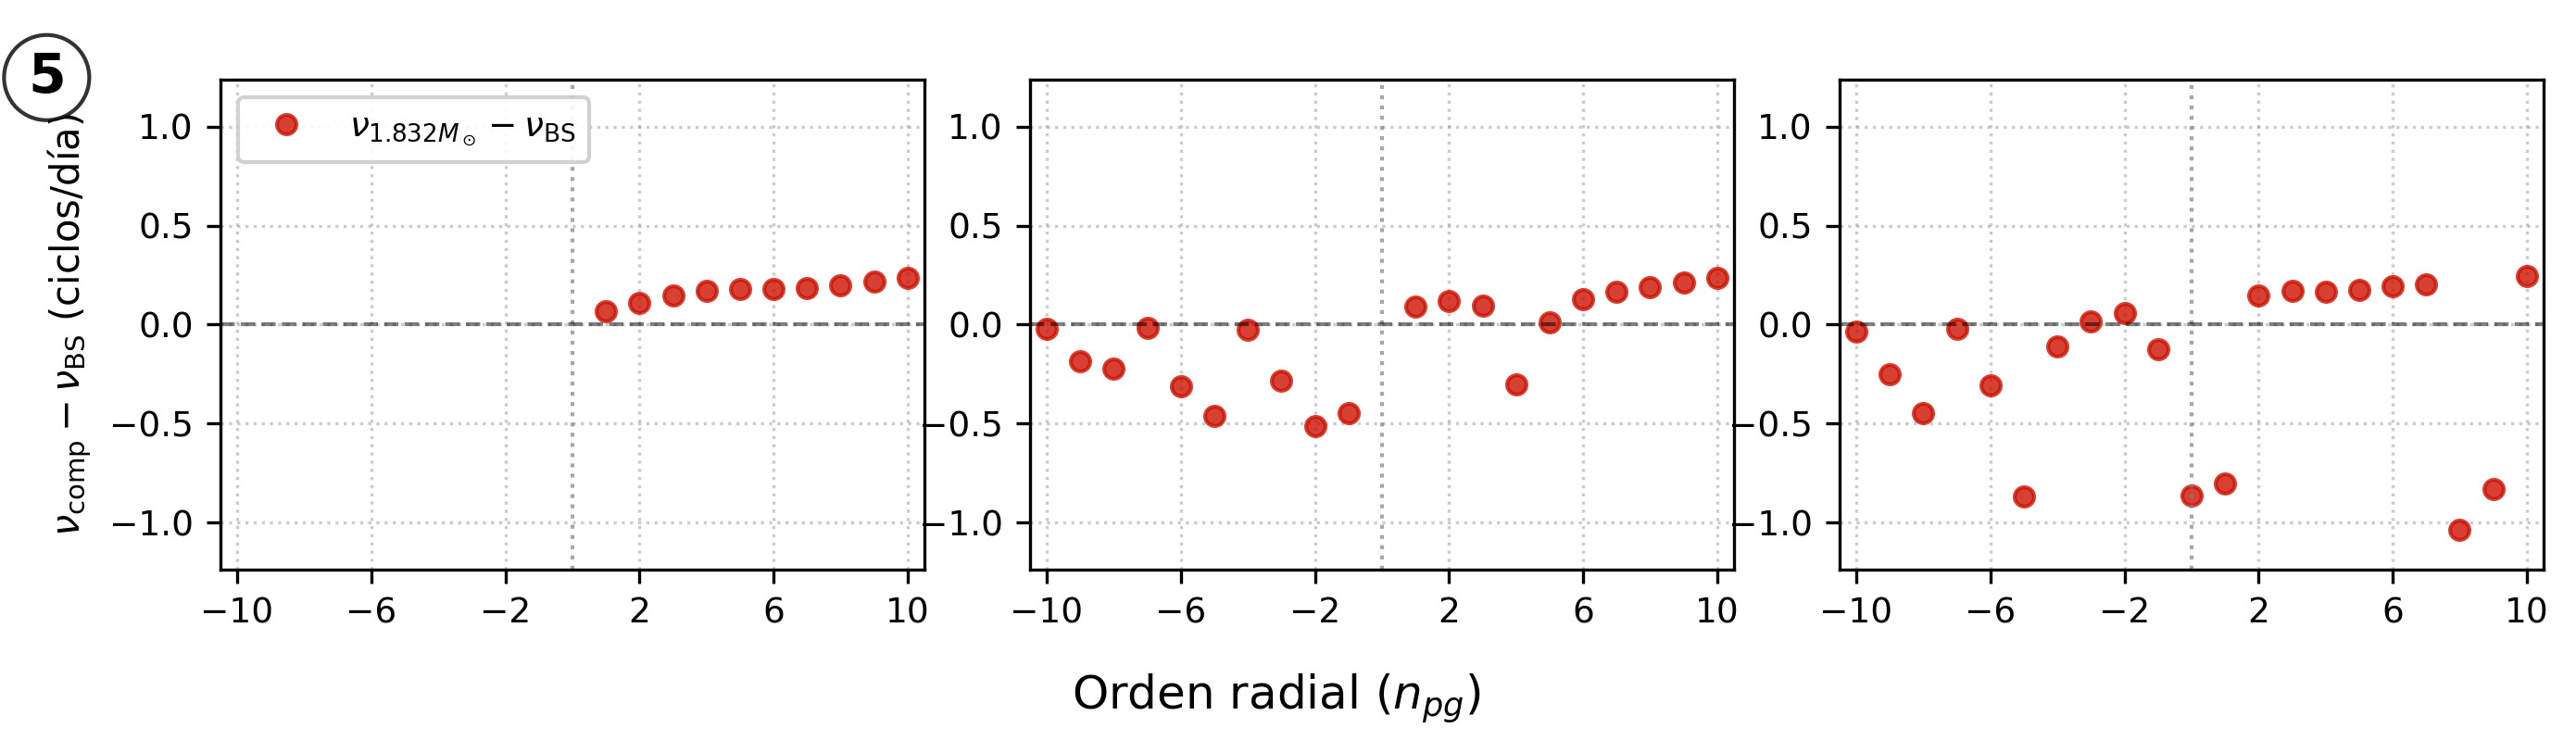
\includegraphics[width=\linewidth]{Imagenes/gyre_analysis_hand_picked/gyre_analysis_mass_1.832_pcomp_28_pbs_63_H_14.8.png}
  \label{fig:gyre_analysis_14.8}
\end{figure}

\clearpage
\thispagestyle{plain}
\begin{figure}[H]
  \centering
  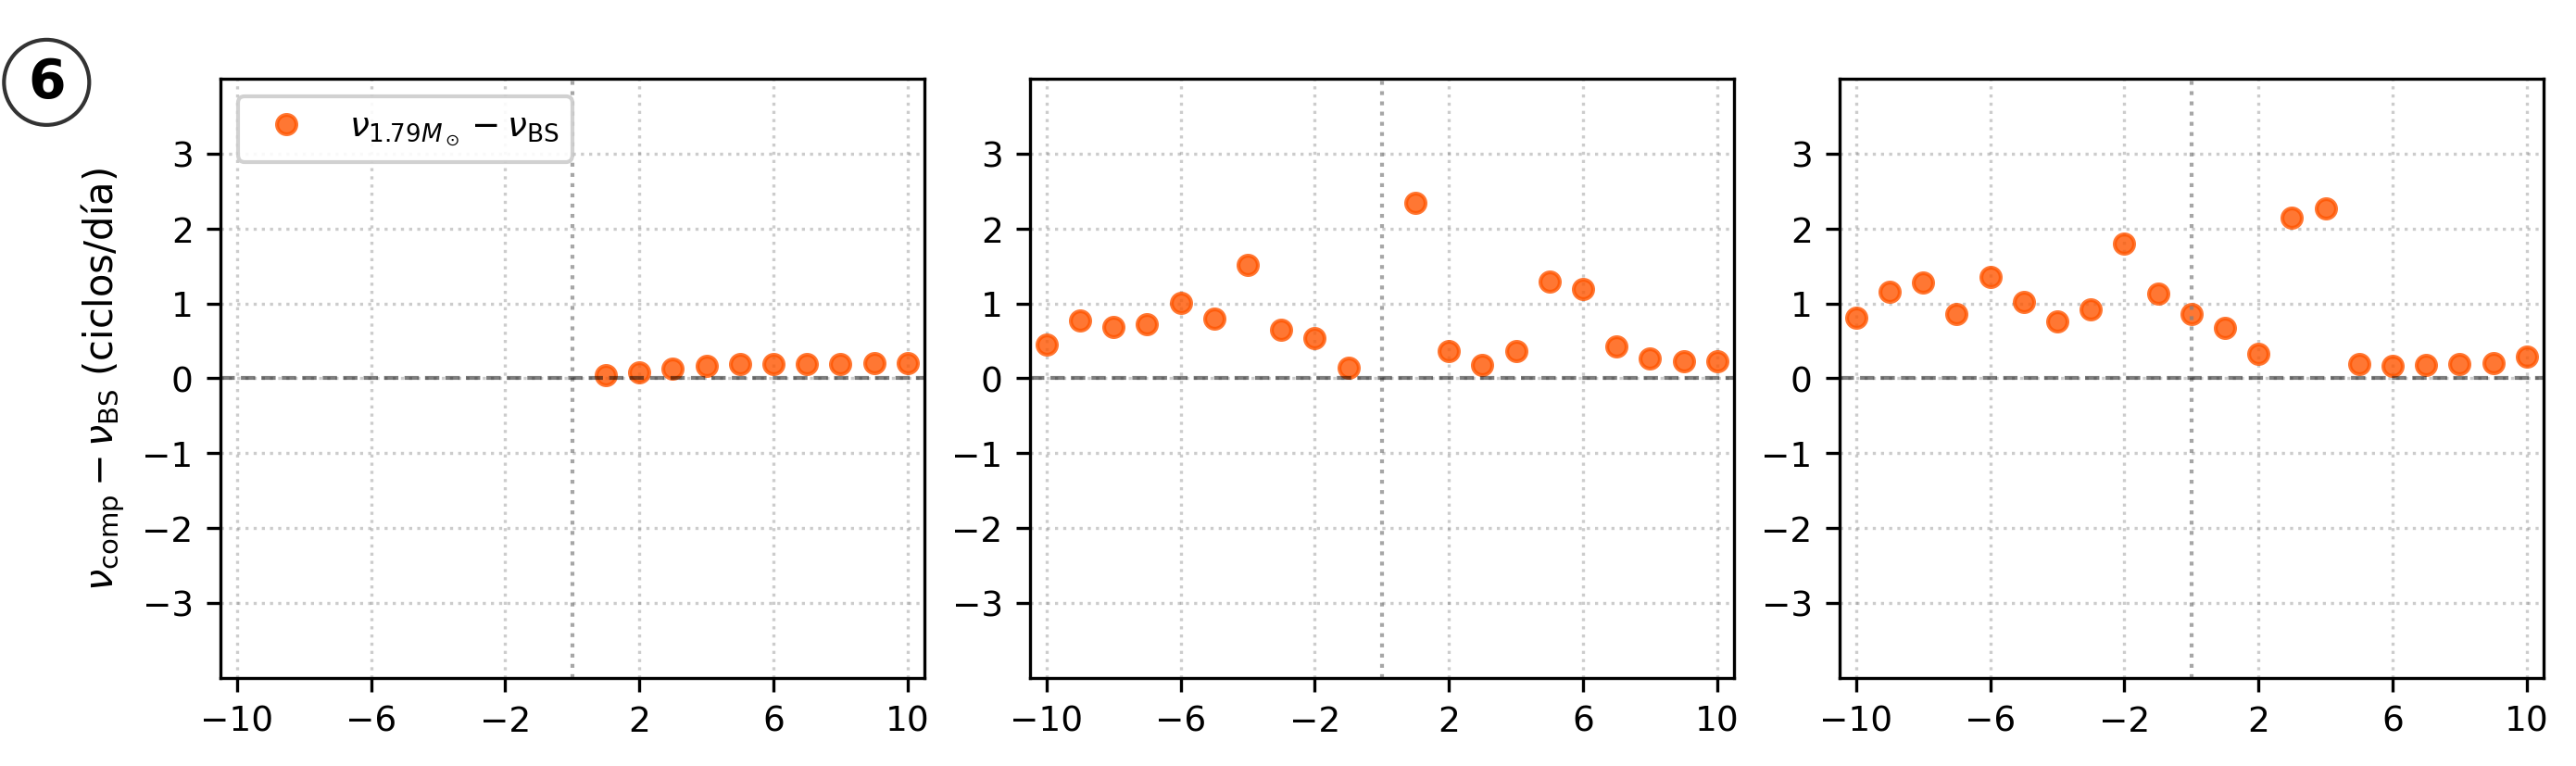
\includegraphics[width=\linewidth]{Imagenes/gyre_analysis_hand_picked/gyre_analysis_mass_1.79_pcomp_38_pbs_72_H_0.8.png}
  \label{fig:gyre_analysis_0.8}

  \vspace{-1.05cm}
  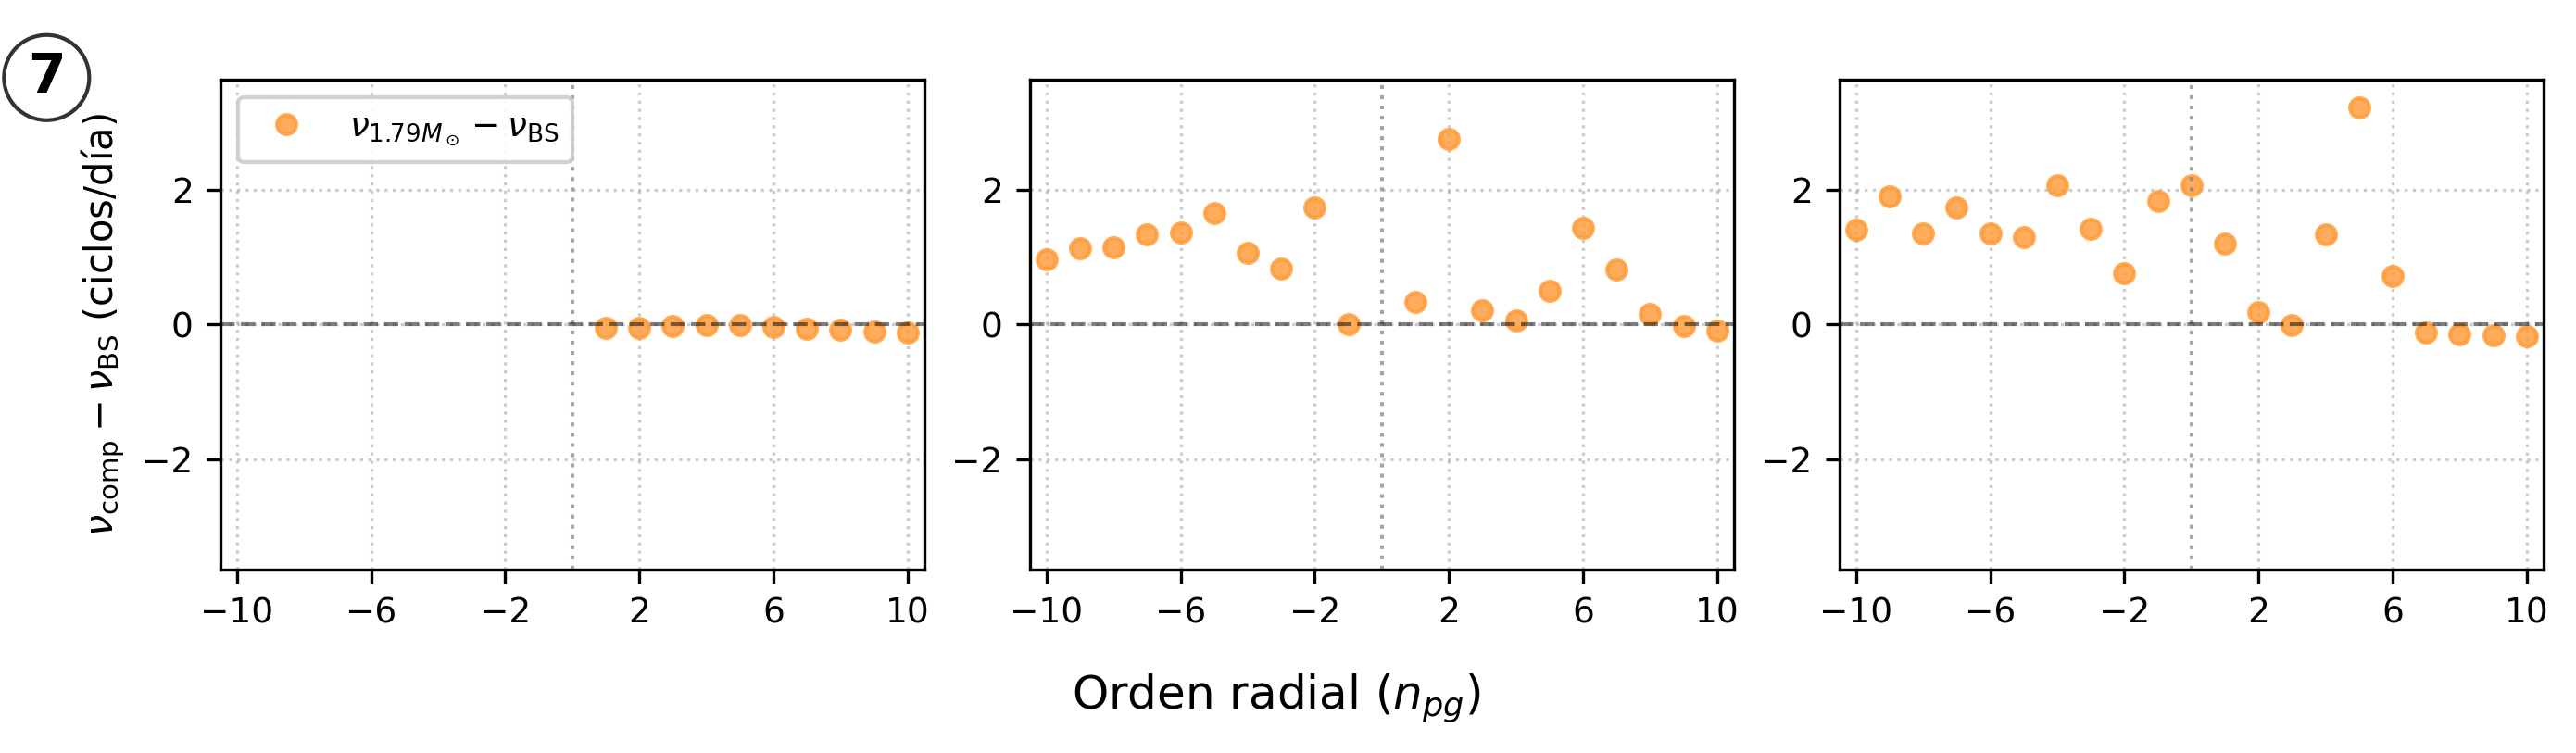
\includegraphics[width=\linewidth]{Imagenes/gyre_analysis_hand_picked/gyre_analysis_mass_1.79_pcomp_45_pbs_92_H_0.1.png}
  \label{fig:gyre_analysis_0.1}
  \vspace{-0.5cm}

  \caption{}
\end{figure}

\clearpage
\restoregeometry